\documentclass[preprint, review, 12pt]{elsarticle}

\usepackage{lineno,hyperref}
\usepackage{amssymb}
\usepackage{url}
\usepackage{paralist}
\usepackage{booktabs}
\usepackage{colortbl}
\usepackage{gensymb}
\usepackage{soul}
\usepackage{nicefrac}

\definecolor{DarkRow}{rgb}{1.0, 1.0, 0.93}
\modulolinenumbers[5]

\journal{Energy}

%%%%%%%%%%%%%%%%%%%%%%%
%% Elsevier bibliography styles
%%%%%%%%%%%%%%%%%%%%%%%
%% To change the style, put a % in front of the second line of the current style and
%% remove the % from the second line of the style you would like to use.
%%%%%%%%%%%%%%%%%%%%%%%

%% Numbered
%\bibliographystyle{model1-num-names}

%% Numbered without titles
%\bibliographystyle{model1a-num-names}

%% Harvard
%\bibliographystyle{model2-names.bst}\biboptions{authoryear}

%% Vancouver numbered
%\usepackage{numcompress}\bibliographystyle{model3-num-names}

%% Vancouver name/year
%\usepackage{numcompress}\bibliographystyle{model4-names}\biboptions{authoryear}

%% APA style
%\bibliographystyle{model5-names}\biboptions{authoryear}

%% AMA style
%\usepackage{numcompress}\bibliographystyle{model6-num-names}

%% `Elsevier LaTeX' style
\bibliographystyle{elsarticle-num}
%%%%%%%%%%%%%%%%%%%%%%%

\begin{document}

\begin{frontmatter}

\title{Scalable Tuning of Building Models to Hourly Data}

\author[atr:garrett]{Aaron Garrett} %%The superscript ``a'' and ``b'' should be in italic.
\author[atr:new]{Joshua New\corref{cor}}
\cortext[cor]{Corresponding author at Oak Ridge National Laboratory; \emph{Email address}: newjr@ornl.gov}

\address[atr:garrett]{Mathematical, Computing, and Information Sciences, Jacksonville State University, Jacksonville, AL, USA}
\address[atr:new]{Oak Ridge National Laboratory, Oak Ridge, TN, USA}


\begin{abstract}
Energy models of existing buildings are unreliable unless calibrated so that they correlate well with actual energy usage. Manual tuning requires a skilled professional and is prohibitively expensive for small projects, imperfect, non-repeatable, and not scalable to the dozens of sensor channels that smart meters, smart appliances, and sensors are making available. A scalable, automated methodology is needed to quickly, intelligently calibrate building energy models to all available data, increase the usefulness of those models, and facilitate speed-and-scale penetration of simulation-based capabilities into the marketplace for actualized energy savings. The ``Autotune'' project is a novel, model-agnostic methodology that leverages supercomputing, large simulation ensembles, and big data mining with multiple machine learning algorithms to allow automatic calibration of simulations that match measured experimental data in a way that is deployable on commodity hardware. This paper shares several methodologies employed to reduce the combinatorial complexity to a computationally tractable search problem for hundreds of input parameters. Accuracy metrics are provided that quantify model error to measured data for either monthly or hourly electrical usage from a highly instrumented, emulated-occupancy research home.
\end{abstract}

\begin{keyword}
Autotune, EnergyPlus, calibration, optimization, evolutionary computation
\end{keyword}

\end{frontmatter}

%\linenumbers

\section{Introduction}
\label{sec:introduction}
Sustainability is perhaps the defining challenge of our time. With only 4.4\% of the world's population, the United States (US) consumes 19\% of the world's primary energy production. Buildings account for the largest fraction of energy consumption in the US, accounting for 41\% of the primary energy used in 2010 \cite{cit:doe2012a}. Building energy model creation and simulation have many uses, but they are often fiscally infeasible for all but the largest projects because of the time required to create a model of an existing building and calibrate it to measured data. The US Department of Energy's (DOE) Building Technologies Office is assisting the development of several Emerging Technology applications to significantly reduce costs and drive simulation-informed actualized energy savings into existing light commercial and residential buildings to meet the US goal of reducing building energy use by 50\% by 2030 compared with a 2010 baseline.

Many simulation-based analysis tools are available \cite{cit:doetools2012} to project how specific policies or energy retrofit measures \cite{Chidiac20115037} would maximize return-on-investment for government and utility subsidies. These tools can help resolve issues such as principle-agent, first cost, and cost/performance trade-offs, as well as maximizing financial metrics such as net present value and simple payback. As with all software tools, their analysis suffers from ``garbage in, garbage out.'' This is complicated by the fact that, unlike cars or planes built to a strict engineering specification, buildings are currently based on one-off designs and constructed in the field. They can last decades or hundreds of years, and rarely do any energy use data exist beyond utility bills. For older buildings, optimal retrofit packages and similar analyses are calculated for a fictitious building and necessarily yield suboptimal results. A central challenge in building energy efficiency is being able to realistically and cost-effectively model existing buildings. Even coarse models are useful to determine how incremental energy conservation measures affect whole-building energy consumption. Their usefulness is dramatically greater for existing buildings, for which existing data can be used to calibrate the energy model. However, differences between models and actual monthly utility bills on the order of 24--97\% \cite{cit:earthadvantage2009,cit:roberts2012} are common. Many measurement and verification (M\&V) protocols specify a required accuracy for a model to be legally useful. Most large organizations use ASHRAE Guideline 14, 5.3.2.4.f requirements, which specify a coefficient of variance for root mean squared error (RMSE) of \textless 15\% or 30\% and a normalized mean bias error of \textless 5\% or 10\% for calibrating to monthly or hourly data, respectively \cite{cit:ashrae2002}.

Several simulation engines, and tools that leverage them, are actively supported by DOE \cite{cit:doetools2012}. DOE’s flagship simulation engine is EnergyPlus \cite{cit:energyplus}, which has been supported with over \$65 million since 1995. OpenStudio \cite{cit:nrel2012} now serves as the primary middleware between simulation engines and analysis tool applications. High-level graphical interfaces and low-level, text-based files allow a user to provide information that fully describes a given building and from which EnergyPlus can calculate detailed heat flow and energy usage information for the building. The number and instances of these input parameters are extensive and highly variable in their combinatorial effects, and their sensitivities are not yet fully explored. This relegates simulation calibration to an ``art,'' and only a few hundred people have qualified for ASHRAE's building energy modeling professional certification. It is unrealistic to expect even an advanced user to be able to provide accurate values for each of the approximately 3,000 parameters expected by EnergyPlus for the average building. To mitigate such issues, a reference or template building already in the preferred tool, which is similar to the user's own building, is used as a default point for parameter values. These values are then ``corrected'' to more closely match the actual building under consideration, depending on the level of information available (e.g., the data specified by an ASHRAE level 1, 2, or 3 audit). In addition, average material properties are typically used from the \textit{ASHRAE Handbook of Fundamentals} (HoF) which is beginning to include significant variances in material properties identified from controlled laboratory tests \cite{cit:ashrae2013}.

As the variance in material properties increases; as building systems, equipment, and materials become more complicated and diverse; and as energy simulation modeling algorithms evolve to more thoroughly model existing systems and capture new equipment technologies, there is a need to mitigate this complexity by relying on cost-effective, intelligent algorithms to calibrate building energy models to use as many data as are available. The Autotune project \cite{cit:new2012} aims to solve this need with an automated process and has previously demonstrated calibration results for envelope parameters using monthly utility data \cite{cit:garrett2013}. This paper extends that work by discussing the scalable methodologies used to tune a building energy model's 100+ envelope parameters to whole-building hourly electrical usage data.

\section{Background}
\label{sec:background}

\subsection{Autotune Background}
The Autotune project has used 269+ channels of 15-minute sensor data from a robotically-emulated-occupancy ZEBRAlliance \cite{cit:miller2012,cit:biswas2012} 2800 ft$^2$ research home. Parametric ensemble models of this building were simulated using high performance computing (HPC). The Titan supercomputer at Oak Ridge National Laboratory (ORNL) allowed the use of 131,072 cores to calculate 524,288 simulations and write 44 TB of data to disk in 68 minutes \cite{cit:sanyal2013a}. Some of the latest advances in web-oriented database storage were used to allow queryable simulations generated from varying 156 inputs and reporting 96 outputs at 15-minute resolution (35 MB per simulation) for 8 million EnergyPlus simulations \cite{cit:sanyal2013b}. Measured data often are corrupt because of  uncalibrated sensors or missing data, so statistical techniques have been refined for autonomous quality assurance and gap-filling \cite{cit:castello2012}. Extensive big data mining was conducted through the creation of an HPC-enabled suite of machine learning algorithms (MLSuite \cite{cit:edwards2013}) to generate agent-based encapsulation of knowledge for Autotune deployment on mobile devices. EnergyPlus was approximated with machine learning algorithms to reduce simulation runtime from 3 minutes to 4 seconds with a minimal trade-off in accuracy for the processed building types \cite{cit:edwards2013}. The Autotune project, to promote open science, is making a portion of the 267 TB (26.9 trillion data points) of EnergyPlus simulation data freely available online\footnote{\url{http://autotune.roofcalc.com}}.

\subsection{Simulation Accuracy}
Despite the proliferating use of building energy tools, there remain many concerns and shortcomings applicable to all simulation engines. The primary concern is typically the accuracy of the simulation engines for realistically modeling (via inputs) a virtual building so that it matches a real-world building. A Home Energy Rating System (HERS) study in 1999 \cite{cit:pigg2001} using the REM/Rate
simulation engine for 2,300 homes in Wisconsin found that the median home's heating use---40\% of the average annual Wisconsin energy bill---was overestimated by 22\%, with the worst 15\% median being off by 62\%. Another study in 2000 \cite{Stein2000339} covering 500 homes in 4 states found no relationship between asset ratings and energy consumption. A 2008 pilot study \cite{cit:earthadvantage2009} found 190 Home Energy Saver, REM/Rate, and SIMPLE residential simulation models had a 25.1--96.6\% error rate compared with actual monthly electrical energy usage. A 2012 study \cite{cit:roberts2012} found that 859 residential models across Home Energy Saver, REM/Rate, and SIMPLE had a mean absolute percentage difference of 24\% compared with actual monthly electrical energy use and of 24--37\% compared with actual natural gas use for a sample size of 500 houses. All of these studies use comparisons with monthly utility bill data; the challenge of accurately matching hourly or 15-minute data for dozens of sub-metered data channels is significantly more difficult.

The challenge for simulation accuracy can be reduced to two primary issues: \begin{inparaenum}[(1)]
\item a gap between the as-modeled and as-built structure, and 
\item limitations of the modeling engine's capabilities.
\end{inparaenum}

\subsection{Common Errors with Simulation Inputs}
Gaps between as-modeled and as-built structures have many sources, with the fault being traceable to an inaccurate input file rather than the simulation engine itself. We have worked with building scientists and conducted a sensitivity analysis to identify the most important input parameters.

Infiltration---the rate at which air and energy flow through the building envelope (typically measured in cubic feet per minute per square foot)---cannot be cheaply tested. Blower-door tests can determine the infiltration rate at a given pressure (usually 50 Pascals), but these are one-time measurements that vary significantly as a function of other variables such as temperature, wind speed, and wind direction. Therefore, infiltration is often one of the first variables energy modeling experts use to manually align a simulation model with actual data.

A second issue is the schedule of building usage, which includes the number of occupants; times of occupancy; heating, ventilation, and air-conditioning (HVAC) set points; operation schedule; and other factors. These also constitute inputs to the simulation engine but are often specified in a separate EnergyPlus file for convenience. For many of these, cost-effective sensors do not exist or are not typically deployed in a building (especially sensors providing data that are easily leveraged by energy modelers). In many cases, estimates of occupancy schedules and relatively static set point temperatures are estimated and then used later to ``true-up'' the simulation to match whole-building data without regard to the accuracy of the actual HVAC thermostat set points.

A third component that modelers often do not use, but which is a major contributor to model variance, is material properties used within a building model. Modelers typically use material properties from the ASHRAE HoF, which relates the average value of a physical property (e.g., conductivity, thermal absorptance) for a given material (e.g., gypsum board, glass fiber insulation, plywood) based on standard tests. Occasionally, the manufacturer labels on materials give more reliable estimates than the average values found in the HoF. However, hotbox testing of specific materials has shown significant variance in materials even from a single manufacturer. Although many of these values are used to update HoF numbers over time, data have traditionally not been reported for variance.  In such cases, energy modelers have few reliable data on which to base the precise values necessary to create an accurate model of material properties for the construction of an individual building.

A fourth gap is that energy modelers typically use building design, building information model files, or similar documents; but craftsmanship influences how those designs are implemented (e.g., a contractor might neglect to put insulation in a corner wall). Many other gaps exist, and most of them persist because business models find saving relatively cheap energy an inadequate incentive to justify the energy modeling expense. For example, the Federal Energy Management Program (FEMP) has rigorous M\&V guidelines \cite{cit:femp2008}for calibrating a model. A financial analysis of 26 FEMP-related energy service company projects on commercial buildings showed that project development costs involving simulation ranged from 10 to 45\% of the total cost for projects smaller than \$1 million. This increased risk (and associated cost) prohibits financing for traditional, simulation-informed calibration and optimization of building retrofits for all but the largest building renovation projects.

\subsection{Common Errors with Simulation Algorithms}
The limitations of engine modeling capabilities are a well-understood, active issue for funded development teams or active communities behind popular simulation engines and tools. There often is a backlog of hundreds of user requests involving the inaccuracies of specific algorithms. The development of a capable software engine applicable to the entire US building stock would result in significant market incentives and policy impacts. Simulation engines are often used to inform policy decisions regarding cost-effectively meeting national energy goals. Although several companies have developed simulation engines closely tied to their product lines, an increasing number are either using co-simulation or switching to large simulation engines like EnergyPlus. However, a few primary factors should be considered regarding the inaccuracies of simulation engines.

First, most simulation engines are engineering models that attempt to model the underlying physics involved in energy consumption. Engineering algorithms are necessarily an approximation of reality (e.g., they use 1-dimensional heat transfer processes because 3-dimensional transfer would take too long to calculate). Some simulation engines allow users to select the needed level of precision on an algorithmic level to allow customization for a particular area of interest. Statistical models show some promise, but they are more useful for normative-based models for policy decisions than for product-level or system-level building modifications. 

Second, there is a lag between the development of innovative technologies and the capability to accurately model them within a simulation engine. Only the most active simulation engine development teams can keep up with, or foresee the need to model, building products, components, or systems before they achieve a significant market share. As the code base grows, so does the challenge of maintaining a software architecture that can accommodate new, integrated technologies (which may impact several parts of a building). Third, virtually all known simulation engines are single-threaded; only recently have attempts been made to leverage traditional multi-core and graphical processing unit computational hardware. Given the significantly different multi-threaded software development paradigms, it is difficult to scale additional simulation capabilities without an increase in runtime for models using them. Fourth, the computer, itself an approximation engine, can provide only limited accuracy in a unit of time for a given algorithm. Most simulation engine development focuses on a reactive process of building a tool sufficient to meet a small fraction of the needs expressed by users.

The Autotune project \cite{cit:new2012} goal is to create an automated process for tuning simulation inputs so that simulation output matches measured data. This repeatable, transferable, scientifically rigorous process can address inaccuracies in both input and algorithms by 
\begin{inparaenum}[(1)]
\item adapting a model to more closely match real-world data from the as-built structure,  and 
\item doing so in a way that accommodates inaccuracies in the underlying engineering
model.
\end{inparaenum}

\subsection{Tuning of Building Models}
Although inaccurate models can be useful in comparative analysis, calibrated models are more useful and often must meet specific calibration criteria to be legally permitted for use in a specific context. To satisfy these requirements, modification of simulation algorithms to address the mismatch (often by working around limitations of a given simulation engine) remains one of the most tractable methods used by experts. This tuning process remains an ``art'' that even the practitioners usually do not enjoy. Practitioners often use infiltration and schedules as the primary ``knobs'' for tuning the simulation to measured data. Properties of the many materials alone provide hundreds more ``knobs.'' Hence building model calibration is a severely under-determined problem with thousands of inputs that can be varied to match potentially only 12 data points, leading to questions as to the physical realism of the final tuned model compared with the large number of valid models. As a starting point, this paper focuses on the most important task of getting the thermal characteristics of the envelope right by tuning envelope properties to match electricity consumption throughout the building.

Initial attempts to develop self-calibrating energy models began around the early 1980s. Many such efforts can be found for individual simulation tools, such as ESP-r \cite{Strachan2008601} while others propose multi-engine frameworks to calibration for sub-components of a building's dynamics \cite{Murphy2013484}. It has also been applied for calibrating calibrating residential energy user to regional data while explicitly taking into account uncertainty \cite{vanRuijven2010269}. Much of the history and previous approaches are consolidated in ASHRAE report 1051-RP \cite{cit:reddy2006}. A more recent paper by Coakley et al. \cite{vanRuijven2010269} surveys and characterizes multiple calibration techniques.



\subsection{Computational Complexity}
The EnergyPlus whole-building energy simulation engine was consolidated from diverse sources around 1995, with functionality traceable back to DOE-2 and DOE's Building Loads Analysis and System Thermodynamics (BLAST) from the late 1970s \cite{cit:energyplus}. Its original design goals were to provide a more consistent software structure for development and modification, to allow third-party programs and components to easily interface with the core system, and to fully integrate the loads, systems, and plants into the simulation \cite{cit:energyplus}. The workflow for a building modeler using a system like EnergyPlus is to create a building's geometry using external software, layer it with detailed metrics encoding material properties, and add equipment currently in or expected to be in the building, including anticipated operational schedules.

A typical residential building model in EnergyPlus has approximately 3,000 input parameters that must be specified. The search space in such a problem is extremely large. Even if each parameter were a simple binary value (e.g., \emph{yes} or \emph{no}), the search space for a 3,000-parameter building would contain $2^{3000}$ possibilities. This is a best-case scenario; the actual size of the search space is effectively infinite because many of the parameters are continuous-valued. This study relied on building simulation experts to identify 156 input parameters, along with minimums and maximums within which they will be varied. Even with this simplification it would take Titan more than 13.8 billion years to calculate all the necessary EnergyPlus simulations to find the best model for a single residential building. Many of the experiments in this paper discuss algorithms and methods to find near-optimal models in a tractable amount of time on commodity hardware.

\subsection{Evolutionary Computation}
A common approach to such search problems, successfully applied in previous building model tuning work \cite{cit:garrett2013}, is evolutionary computation (EC). EC \cite{cit:dejong1993,cit:spears1993,cit:fogel1994,cit:fogel2000} is a stochastic search algorithm that attempts to mimic biological evolution by maintaining a set of candidate solutions (see Figure~\ref{fig:chromosome}), referred to as a \emph{population}. Each candidate solution is evaluated to determine its \emph{fitness}, a problem-dependent measure of how well it solves the problem \cite{cit:dejong2006}. In essence, the candidate solutions act as samples of the search space, and their fitness values provide an approximation of the gradient. However, unlike strict gradient-based techniques, an EC provides some (typically small) opportunity for less fit candidates to influence the search process, which helps the EC to avoid local optima \cite{cit:michalewicz2004}. 

\begin{figure}[htbp]
\centering
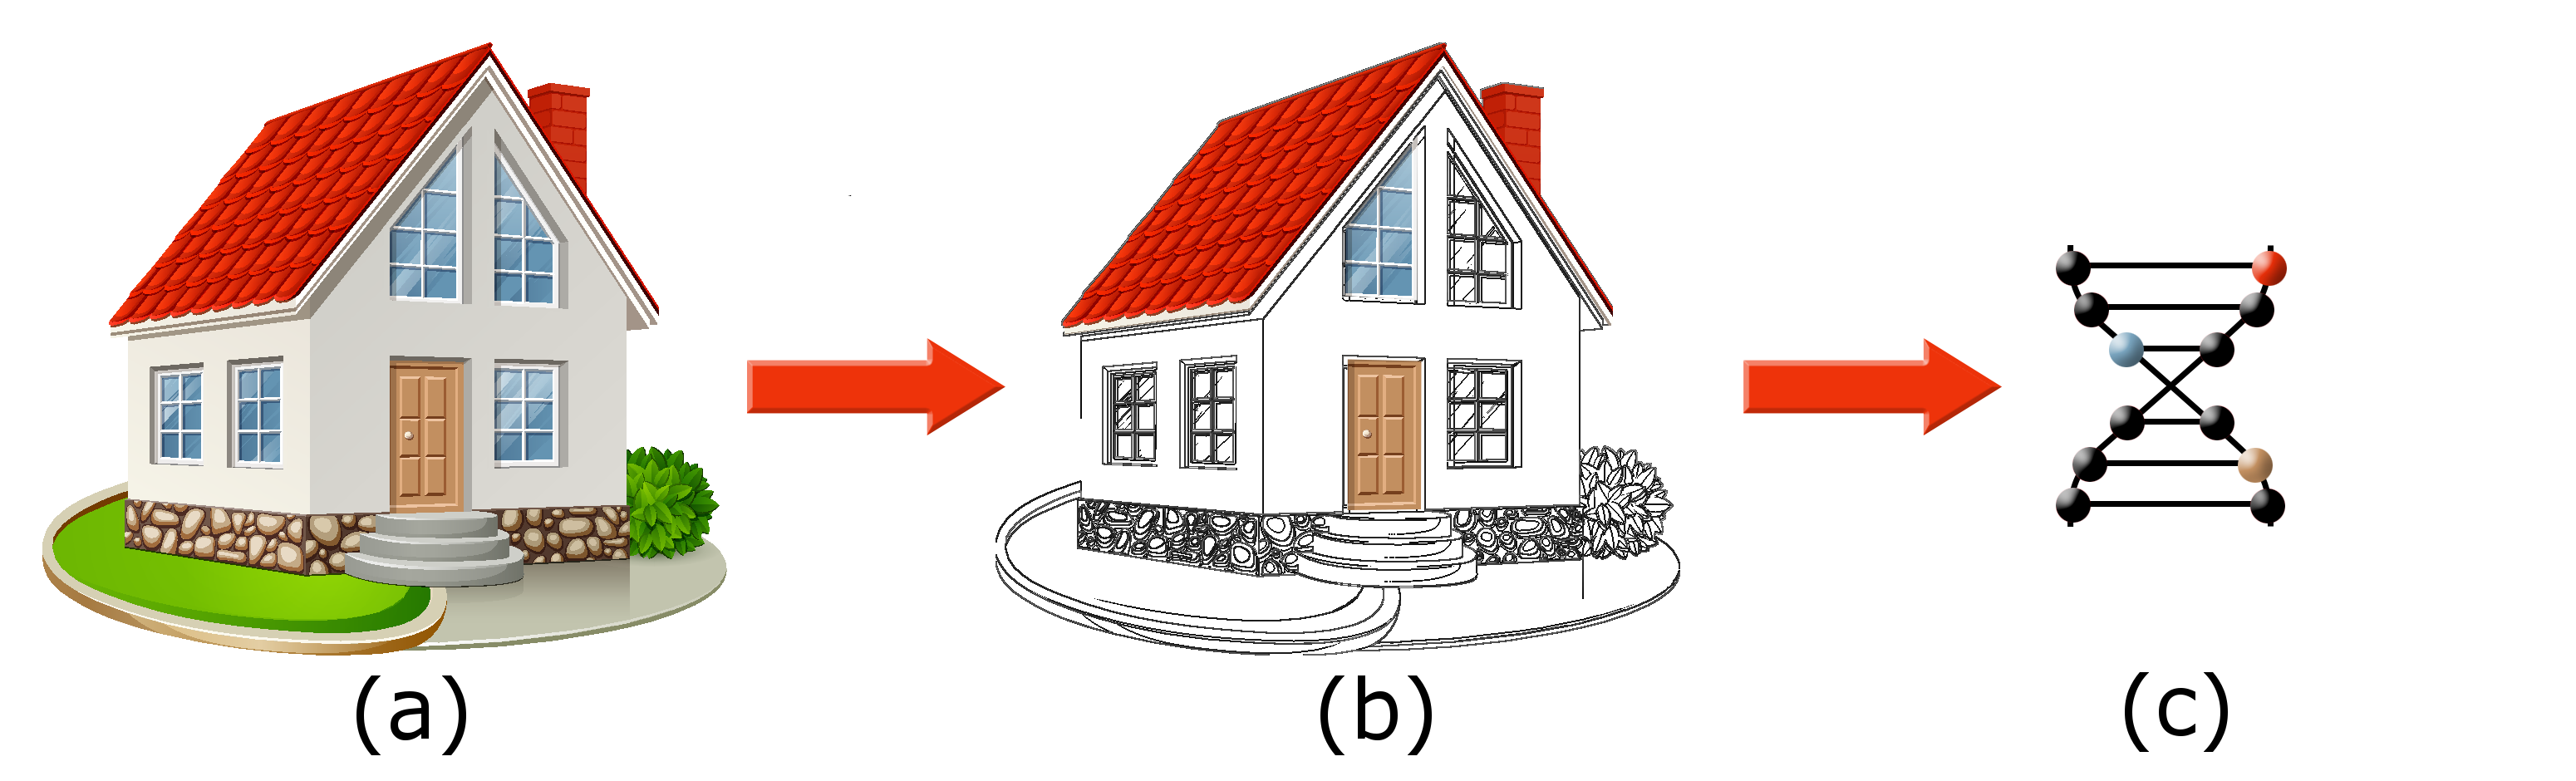
\includegraphics[width=5in]{graphics/autotune_chromosome}
\caption{Candidate solutions represent the essential components of the problem that should be optimized. In the building-model-calibration case, the design of a candidate solution progresses as follows: 
(a) The base model is analyzed to determine optimization variables.
(b) The optimization variables are isolated.
(c) The optimization variables are encoded in some structure that can participate in the evolution (known as the \emph{genotype}).}
\label{fig:chromosome}
\end{figure}

Since EC is a population-based search, it has a number of aspects that are inherently parallel. Most important for this work, each candidate in the population must be evaluated to determine its fitness, and the evaluation of one candidate is typically independent of the others. For expensive evaluation functions, the ability to determine the fitness values of an entire population simultaneously greatly increases the search efficiency. In addition to parallel evaluations, EC approaches called \emph{island models} \cite{cit:eiben2007} maintain multiple populations, each of which performs parallel evolution. In many cases, each island (i.e., isolated population) is allowed to explore a different region of the search space, possibly in different ways. Most island models have mechanisms in place that allow candidate solutions to \emph{migrate} between islands (usually with low frequency), allowing information exchange between the populations.

In the context of this work, a candidate solution is a building with a chromosome represented by a list of building model parameters to be tuned. To evaluate a candidate solution, its corresponding EnergyPlus input data file (IDF) model is constructed and passed to the EnergyPlus simulation engine, producing an entire set of output measures (e.g., heating/cooling loads). These output measures are then compared with actual measured data from the building. The resulting measure of accuracy is used as the fitness value for the candidate solution. 

The interaction among candidate solutions in the population, defined in terms of \emph{evolutionary operators}, drives the evolutionary process. These operators determine how current solutions are recombined or modified to produce new solutions, as well as which solutions get to contribute information to the next generation. Figure~\ref{fig:crossover} illustrates the basic concept of an evolutionary operator (recombination, in this case). The particular evolutionary operators used in this work were heuristic crossover, Gaussian mutation, tournament selection, and generational replacement. Each of these operators is standard in the EC literature, and all were described previously in \cite{cit:garrett2013}.

\begin{figure}[htbp]
\centering
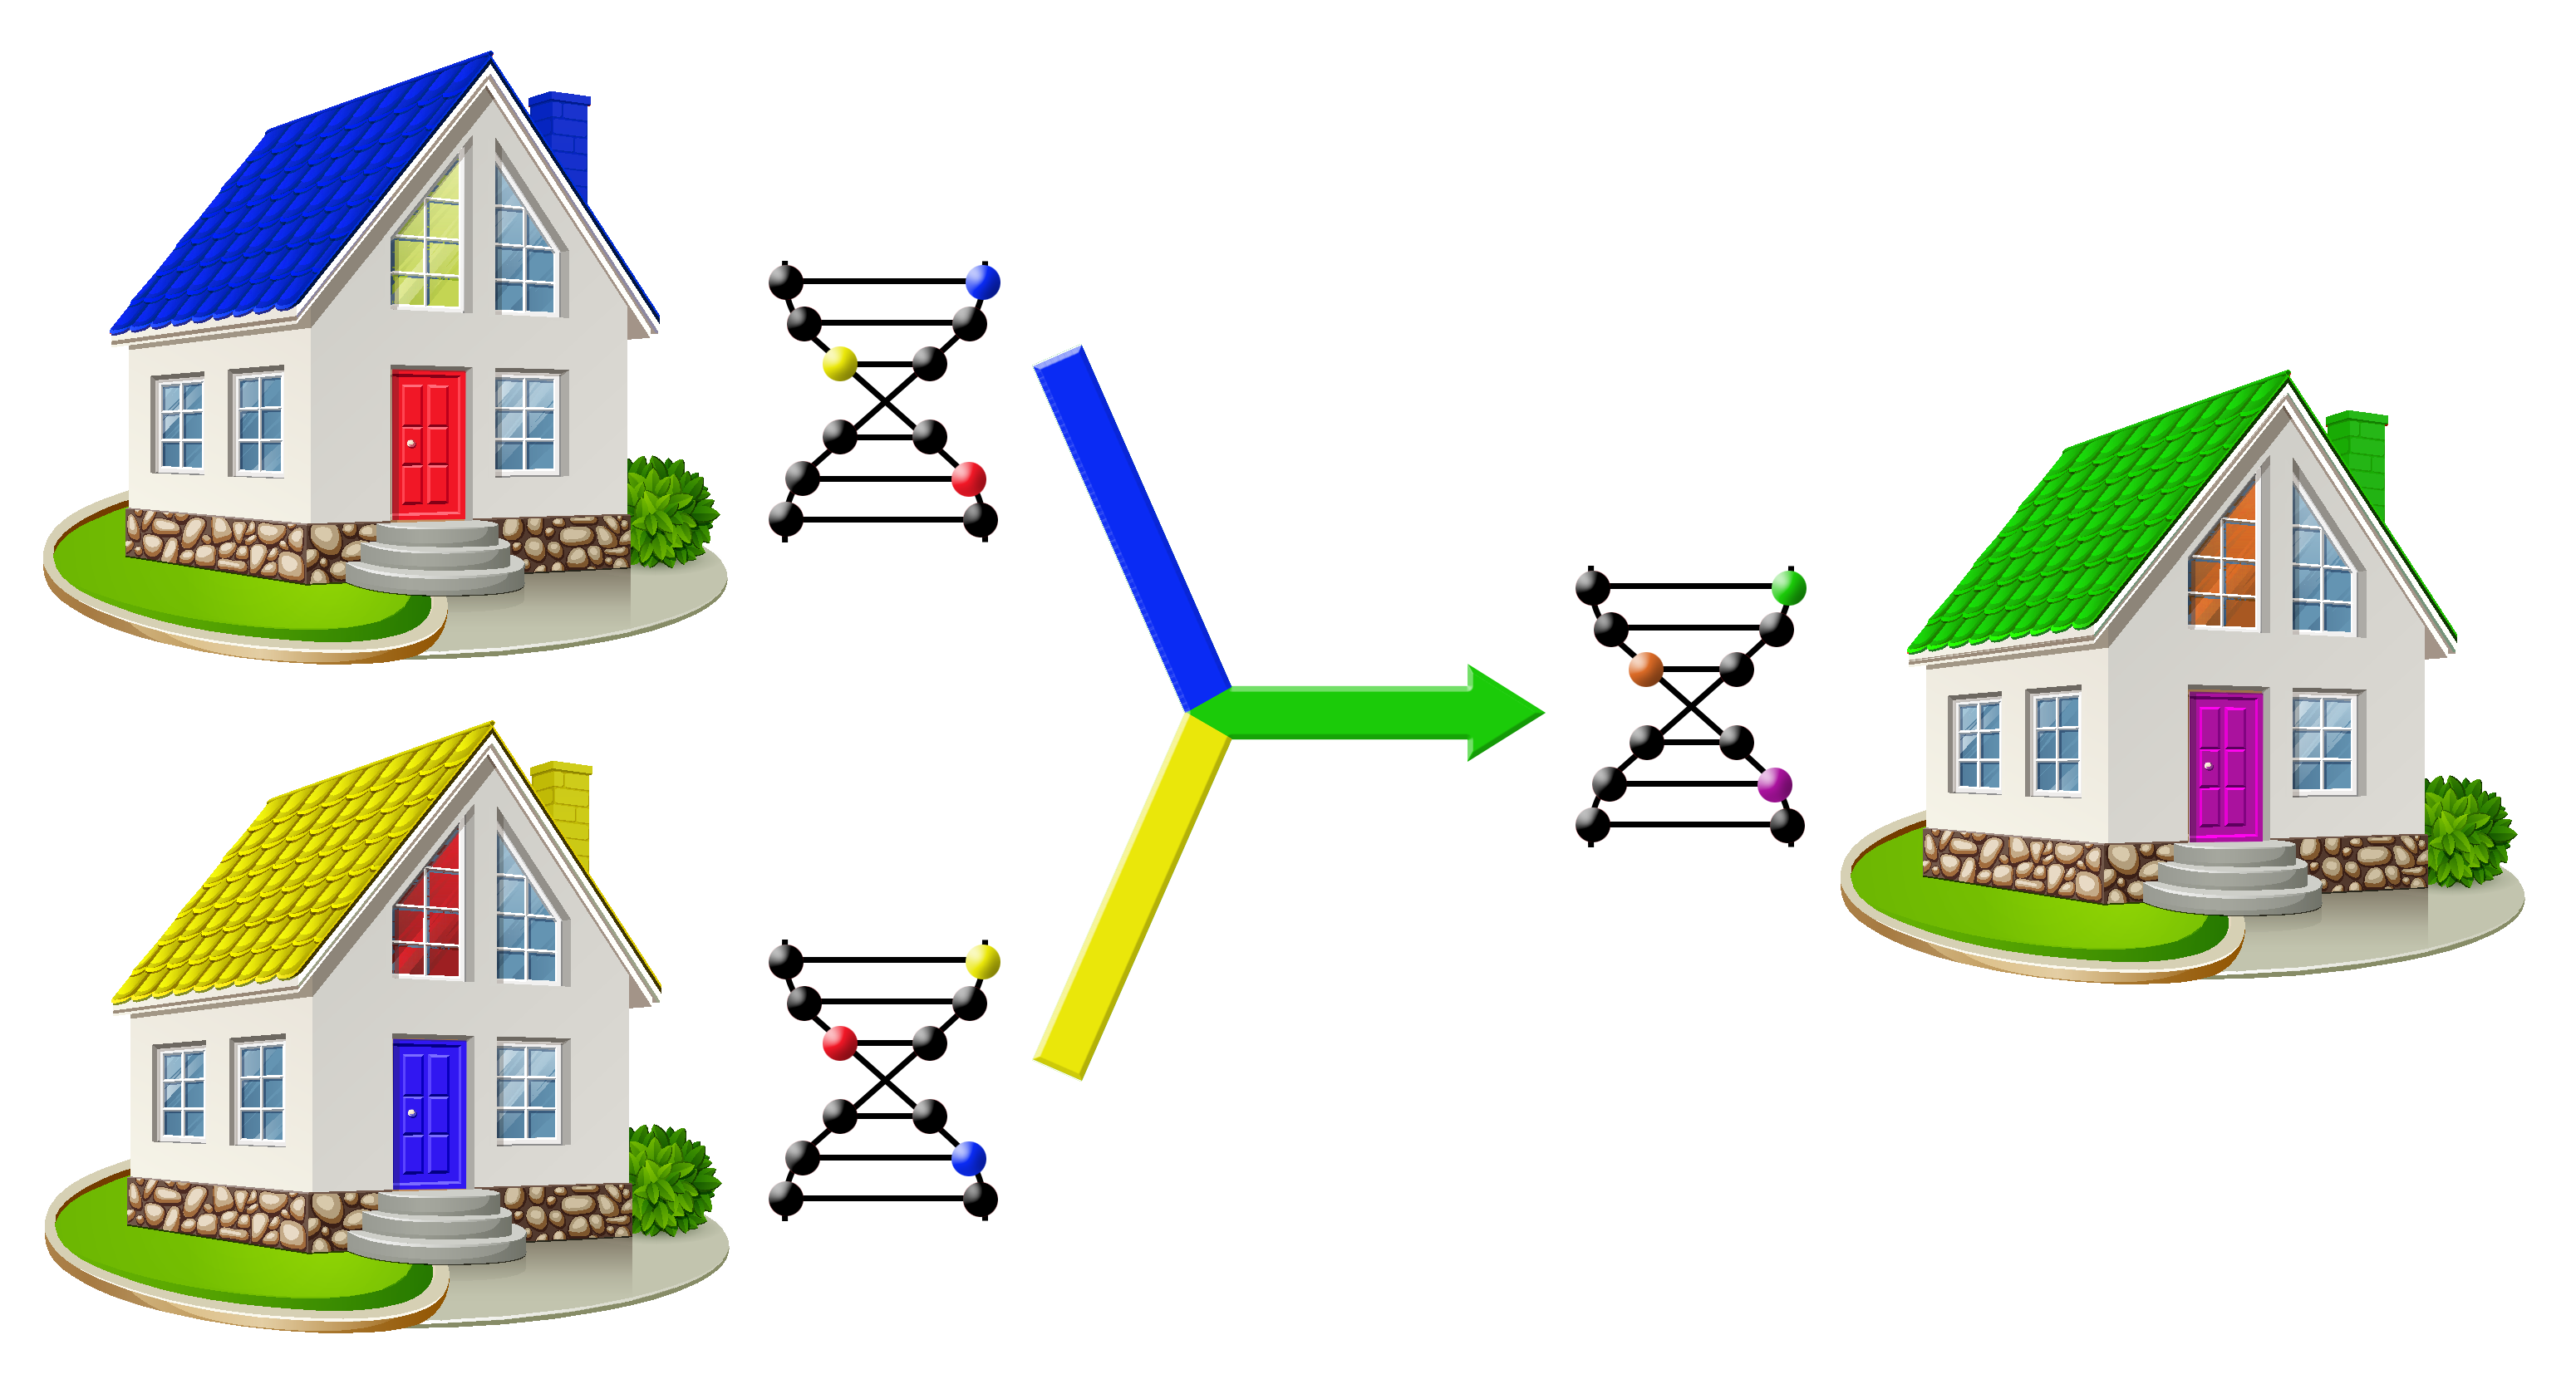
\includegraphics[width=5in]{graphics/autotune_crossover}
\caption{Evolution progresses as candidate solutions undergo the effects of evolutionary operators, such as recombination. In this illustration, the two genotypes (blue-yellow-red and yellow-red-blue) are recombined to produce an offspring candidate solution (green-orange-purple). The particular recombination illustrated here through color-mixing is similar to an approach in the EC literature known as \emph{blend crossover}.}
\label{fig:crossover}
\end{figure}


\section{Methodology}
\label{sec:methodology}
Previous work \cite{cit:garrett2013} focused on tuning a building to monthly utility data. The work presented here takes a more ambitious approach by attempting to optimize the match between a model building and actual hourly electricity usage data. The reference building used in this work is house number 1 in the Wolf Creek subdivision (WC1), an ORNL ZEBRAlliance experimental energy-efficient home. This house has a plethora of energy-efficiency technologies: 
\begin{inparaenum}[(1)]
\item standing seam metal roof with infrared reflective pigments to boost solar reflectance,
\item ENERGY STAR appliances, 
\item triple-pane, low-emittance argon-filled windows, 
\item compact fluorescent lighting, 
\item a horizontal ground loop that leverages foundation and utility excavations, 
\item high-efficiency water-to-air heat pump for space conditioning, 
\item high-efficiency water-to-water heat pump for hot water heating, 
\item an energy recovery ventilator to transfer heat and moisture between fresh incoming and outgoing air, and 
\item structurally insulated panel walls filled with expanded polystyrene insulation.
\end{inparaenum}
For more information, see \cite{cit:miller2012,cit:biswas2012}. The house is fitted with more than 300 sensors that collect data at 15-minute timesteps using standard, wired-sensor data acquisition systems.

\subsection{Base Models}
The data, models, and accuracy metrics described in this subsection are an extension of those previously reported in \cite{cit:garrett2013}. In the following experiments, two different model buildings are used. The first model, the \emph{refined} model, was last modified on March 29, 2012. It matches whole-building annual electric consumption exactly, but it has a sum of absolute errors (SAE) of 1,276.34 kWh for monthly and 6,242.04 kWh for hourly electrical data over the entire year. An earlier version of that same model, the \emph{primitive} model was completed on July 28, 2010. It has an SAE of 1,623.36 kWh for monthly and 8,113.69 kWh for hourly electrical data when summed for the entire year. These two baseline models are separated by approximately four person-months of effort over the course of nearly two calendar years, with the refined model being the recipient of that effort.

\subsection{Tuning Parameters}
Only a subset of the real-value parameters of the models, as specified by domain experts, was used as a part of the tuning process; the phrase ``tuning parameters'' refers to these variables. The 156 tunable parameters provided through the project website\footnote{\url{http://bit.ly/autotune_parameters}} are too extensive to list, but most of them are for building material properties. Although these parameters are individual line changes in an EnergyPlus IDF input file, several instances of each material, equipment, and so on may be used throughout a building. The Autotune system currently scales to tune any set of numerical parameters and can be customized for tuning only selected parameters in customizable ways. This allows calibration according to the needs of a particular use case or comparison with manual tuning efforts.

\subsection{Measured Data}
In 2010, the energy consumed by the average US residential building cost \$2,201 \cite{cit:doe2012a}. On average, 53.9\% of that energy went to space conditioning \cite{cit:doe2012b}, which accounted for 42.9\% of the cost and amounted to \$944/year. The energy-efficient HVAC system in WC1, in contrast, actually cost \$472.62 for January 1--November 30, 2010. This 50\% cost reduction for an energy-efficient home serves as a reference point for the tuning results presented throughout the residential study.

For the all-electric WC1, actual energy usage data for all HVAC equipment were reliably collected from January 1 through November 28, 2010, at which point a new set of test HVAC equipment was installed. Therefore, in all experiments reported, the ``yearly'' electrical usage (and likewise the ``full'' schedule) always refers to the electrical usage from January 1 to November 28. The electrical usage in this work was calculated as the sum of all of the heating and cooling ideal loads for every time period (in kilowatt-hours).

\subsection{Tuning Accuracy}
In the following experiments, the primary metric used for measuring tuning accuracy is the SAE\footnote{The SAE was chosen as the primary metric, rather than RMSE, for example, because of its ease of interpretation in terms of dollar difference.}. The SAE was calculated according to Eq.~\ref{eq:sae}, where $M_i$ is the heating+cooling load of the model and $A_i$ is the heating+cooling load of the actual ZEBRAlliance WC1 building. This equation contains only  $n=8016$ hours because actual data were not collected for December; this value is indicated as $SAE_{hour}$. One of the acceleration methods used is to tune on an abbreviated schedule of only 4 days (January 1, April 1, August 1, and November 1) before transitioning to a full year; use of this variant of the metric is indicated as four-day SAE.

\begin{equation}
\label{eq:sae}
	SAE = \sum_{i=1}^{n}\left|M_i - A_i\right|
\end{equation}

One practical consideration in moving from monthly to hourly data is that failures and sensor drift are more prevalent and easily detectable in hourly data. For this dataset, it was found that sensors failed to make a measurement in approximately 2\% of all measurements. In \cite{cit:garrett2013}, in dealing with error calculations, the failures were treated as 0 values in the summation because it was believed they would not significantly impact monthly usage. For hourly data, however, they make a fourfold larger difference, and it was decided to ignore any hour that contained at least one sensor failure (approximately 8\% of the data).

\subsection{Evolutionary Computation Parameters}
The following experiments always use 1,024 fitness evaluations (EnergyPlus simulations compared with actual data) to allow comparison across experiments. These evaluations are organized into 16 individuals (building models) evolved over 64 generations, tournament selection with tournament size 4, generational replacement with weak elitism (one elite), heuristic crossover, and Gaussian mutation with a usage rate of 1.0 and a mutation rate of 10\% of the allowable range of each variable, unless otherwise specified. Because of the stochastic nature of this approach, results are shown for eight independent trials.



\section{Experiments}
\label{sec:hourly}

\subsection{Experiment 1---Determining a Fitness Surrogate}
\label{sub:experiment1}
An annual EnergyPlus simulation for the WC1 reference building at 1 hour time intervals (over 8,000 time periods) requires 8 minutes of runtime and cannot currently be efficiently parallelized. This type of fine-grained schedule leads to a much more exact, but computationally expensive, simulation. A 4 day simulation has only 96 time periods of output data but can run in seconds. It was also previously established \cite{cit:garrett2013} that tuning on an abbreviated schedule of only 4 days (January 1, April 1, August 1, and November 1) was a defensible acceleration method for monthly data, and this experiment validates the same behavior for hourly data. We do this by establishing a correlation between the error rate of the 4 day and full schedules, which requires a particular kind of sampling spanning from high to low error. An EC was used to minimize the error in the abbreviated schedule, and the hourly error rates in the 4 day and full schedules of each created individual were measured and stored to determine their correlation. To ensure against statistical anomalies, the EC was run four different times with different initial populations each time.

The entire set of 1,024 individuals for each of the four trials is plotted in Figure~\ref{fig:hour-corr}. This plot compares the hourly SAE between the candidate solutions and the actual energy usage, for both the 4 day schedule and the full schedule, for each of the four independent trials. The graph shows a strong linear correlation between the electricity usage with the 4 day schedule and the usage with the full schedule---0.9697, 0.9704, 0.9472, and 0.9382 for each of the four trials, respectively. This can be seen in the first row of Table~\ref{tab:hour-corr}, which shows how the correlation changes as the data focus more on the later generated samples (which would typically have lower SAE). So, as with previous results, the 4 day abbreviated schedule appears to be an acceptable surrogate for the full schedule. 

\begin{figure}[htbp]
\centering
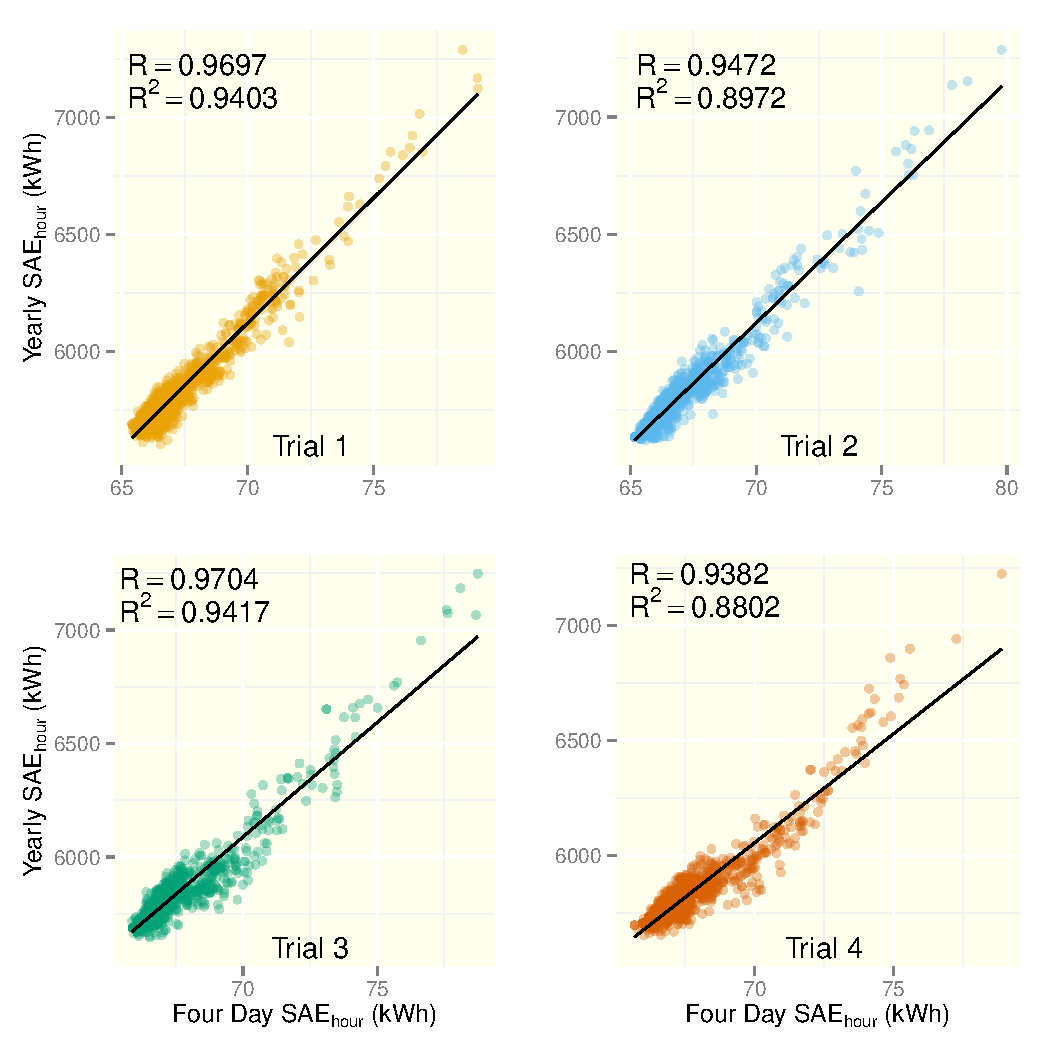
\includegraphics[width=5in]{graphics/figure1.pdf}
\caption{Each of the four independent trials shows a very high correlation between the 4 day and full-year-schedule SAE of hourly electrical usage. This means that an abbreviated surrogate (4 -day schedule) is a plausible method of expediting the tuning.}
\label{fig:hour-corr}
\end{figure}

\begin{table}[htbp]
\centering
\caption{The sampling of the SAE to determine correlation was done using an EC with the objective of minimizing the SAE. This produced initial samples with relatively high SAE values and subsequent samples with generally lower SAE as more data were used. The correlation using only the first $N$\% of the samples produced shows that even the initial samples are strongly correlated most of the time (with the exception of Trial 3).}
\label{tab:hour-corr}
\begin{tabular}{ccccc}
\toprule
Data Used & Trial 1 & Trial 2 & Trial 3 & Trial 4\\
\midrule
100\% & 0.9603 & 0.9422 & 0.9015 & 0.9555\\\rowcolor{DarkRow}
90\%  & 0.8668 & 0.8438 & 0.6545 & 0.8788\\
80\%  & 0.8683 & 0.8573 & 0.6444 & 0.8922\\\rowcolor{DarkRow}
70\%  & 0.8726 & 0.8561 & 0.6231 & 0.8944\\
60\%  & 0.8671 & 0.8489 & 0.6078 & 0.8952\\\rowcolor{DarkRow}
50\%  & 0.8703 & 0.8489 & 0.5557 & 0.8971\\
40\%  & 0.8774 & 0.8417 & 0.5663 & 0.9020\\\rowcolor{DarkRow}
30\%  & 0.8794 & 0.8208 & 0.6015 & 0.8973\\
20\%  & 0.8841 & 0.8231 & 0.5988 & 0.8860\\\rowcolor{DarkRow}
10\%  & 0.8796 & 0.8235 & 0.3985 & 0.8714\\
\bottomrule
\end{tabular}
\end{table}


\subsection{Experiment 2---Tuning Using the Abbreviated Schedule}
\label{sub:experiment2}
The abbreviated schedule is desirable since it is significantly less expensive to compute, has proved to be an effective surrogate for full-schedule error, and provides a baseline against which other results can be compared and contextualized. In Experiment 2, we tune the refined and primitive models on hourly electrical usage with the abbreviated schedule. We then use the 4 day tuned models to calculate data for the entire year to get a full-schedule SAE that is directly comparable to other experiments. %Aaron, please confirm this is correct...it took me a little while to remember this fact with paragraph text saying full-schedule but the caption saying abbreviated schedule.

Table~\ref{tab:hourly-abbrev} presents the final population statistics for full-schedule SAE on each model and trial. The actual full-schedule data were compared with each of the 16 candidates in the final population for each trial, and table reports the average and minimum SAE values from this comparison. For the refined model, the average minimum yearly SAE achieved by the EC was 5,660 kWh. This corresponds to a reduction of 582 kWh in SAE---an almost 10\% reduction from the model, which had an SAE of 6,242 kWh. For the primitive model, the average minimum yearly SAE was 7,453 kWh, a reduction of 660 kWh or 8\%. This is also a 35\% reduction in the error between the primitive and refined models (8,114 kWh for the primitive and 6,242 kWh for the refined).


\begin{table}[htbp]
\centering
\caption{In Experiment 2, the EC was used to optimize the primitive and refined models eight independent times (thus, 16 different tunings) using the abbreviated schedule. The final population of 16 individuals for each tuning were used to produce the statistics in this table. The average and minimum $SAE_{hour}$ (kWh) values for electrical usage from the final populations are shown.}
\label{tab:hourly-abbrev}
\begin{tabular}{llcccccccc}
\toprule
 &  & \multicolumn{8}{c}{Trial (kWh)}\\
Model & Metric & 1 & 2 & 3 & 4 & 5 & 6 & 7 & 8\\
\midrule
Primitive & Avg & 7539 & 7578 & 7683 & 7638 & 7495 & 7467 & 7503 & 7587\\\rowcolor{DarkRow}
Refined   & Avg & 5720 & 5708 & 5792 & 5762 & 5750 & 5783 & 5806 & 5698\\
Primitive & Min & 7393 & 7507 & 7595 & 7545 & 7393 & 7360 & 7356 & 7477\\\rowcolor{DarkRow}
Refined   & Min & 5620 & 5625 & 5709 & 5687 & 5640 & 5671 & 5711 & 5616\\
\bottomrule
\end{tabular}
\end{table}


\subsection{Experiment 3---Tuning Using the Full Schedule}
\label{sub:experiment3}
For comparison, this experiment focuses on using the full schedule for tuning the models. This approach is more computationally expensive than using the abbreviated schedule. The only difference between this experiment and Experiment 2 is the use of the full schedule for the EnergyPlus simulation to calculate candidate fitness. The expectation is that this would generate tuned models with lower SAE values compared with actual data.

Table~\ref{tab:hourly-full} displays the final population statistics, the averages and minimums, for the full-schedule SAE on each model and trial. For the refined model, the average minimum SAE across eight trials was 5,539 kWh. Compare this error with that of the baseline file (6,242 kWh) and of the abbreviated schedule EC (5,660 kWh). Clearly, using the full schedule throughout the evolution provides a lower error (by 121 kWh) than using the abbreviated schedule. However, this additional 2\% reduction in error requires more than five times the computational resources. The abbreviated-schedule EC was able to complete a single trial in about 1.5 hours on an eight-core machine, whereas the full schedule EC required 8 hours on the same machine. For the primitive model, the average minimum SAE across eight trials was 7,162 kWh. Once again, this error must be compared with the baseline file (8,114 kWh) and with the abbreviated-schedule EC (7,453 kWh). The result shows a reduction of 291 kWh in SAE from the abbreviated schedule, which corresponds to a 4\% reduction for a similar fivefold increase in computational time.

\begin{table}[htbp]
\centering
\caption{The final population of 16 individuals for each tuning in Experiment 3 were used to produce the statistics in this table. The average and minimum $SAE_{hour}$ (kWh) values for electrical usage from the final populations are shown.}
\label{tab:hourly-full}
\begin{tabular}{llcccccccc}
\toprule
 &  & \multicolumn{8}{c}{Trial (kWh)}\\
Model & Metric & 1 & 2 & 3 & 4 & 5 & 6 & 7 & 8\\
\midrule
Primitive & Avg & 7275 & 7245 & 7250 & 7259 & 7338 & 7202 & 7274 & 7272\\\rowcolor{DarkRow}
Refined   & Avg & 5582 & 5641 & 5620 & 5594 & 5636 & 5623 & 5623 & 5596\\
Primitive & Min & 7175 & 7138 & 7150 & 7122 & 7253 & 7114 & 7162 & 7179\\\rowcolor{DarkRow}
Refined   & Min & 5518 & 5568 & 5527 & 5510 & 5560 & 5550 & 5558 & 5523\\
\bottomrule
\end{tabular}
\end{table}



\subsection{Experiment 4---Tuning Using Both Schedules Serially}
\label{sub:experiment4}
As shown in Experiment 3, the full schedule produces better tuning results but requires more computational resources. If additional resources are allotted, it may be best to employ those after the tuning process has produced a set of faithful models. The EC can be started from a known set of good solutions (which we call \emph{seeds}), permitting tuning in two parts---first with the abbreviated schedule to produce a set of seeds and then with the full schedule to produce the final tuning.

In this experiment, the first 768 E+ simulations were done using the 4 day schedule. At the end of those simulations, the best half (8) of the final population's candidate solutions were inserted as seeds into a new initial population of 16 candidates. (The other 8 candidates were randomly generated.) This population was then evolved for the remaining 256 evaluations on the yearly schedule.

Table~\ref{tab:hourly-serial} shows the final population minimums and averages for each trial for both the refined and primitive models. The average minimum SAE was 5,581 kWh for the refined model and 7,343 kWh for the primitive model. As expected, the performance is better than that using the abbreviated schedule alone (5,660 kWh and 7,453 kWh for refined and primitive models, respectively) but not as good as using the full schedule throughout the evolution (5,539 kWh and 7,162 kWh). The SAE reduction was 79 kWh for the refined model and 110 kWh for the primitive model, corresponding to a movement of 66\% and 38\% toward the full schedule performance for each model. This performance comes at a cost of approximately double the computational expense of the abbreviated schedule only (3 hours instead of 1.5 hours), which is less than the fivefold increase of the full schedule (over 8 hours). 


\begin{table}[htbp]
\centering
\caption{The final population of 16 individuals for each tuning in Experiment 4 were used to produce the statistics in this table. The average and minimum $SAE_{hour}$ (kWh) values for electrical usage from the final populations are shown.}
\label{tab:hourly-serial}
\begin{tabular}{llcccccccc}
\toprule
 &  & \multicolumn{8}{c}{Trial (kWh)}\\
Model & Metric & 1 & 2 & 3 & 4 & 5 & 6 & 7 & 8\\
\midrule
Primitive & Avg & 7404 & 7463 & 7469 & 7467 & 7393 & 7381 & 7434 & 7403\\\rowcolor{DarkRow}
Refined   & Avg & 5626 & 5670 & 5688 & 5614 & 5695 & 5667 & 5642 & 5646\\
Primitive & Min & 7306 & 7382 & 7402 & 7378 & 7328 & 7283 & 7362 & 7306\\\rowcolor{DarkRow}
Refined   & Min & 5564 & 5586 & 5608 & 5545 & 5596 & 5618 & 5566 & 5563\\
\bottomrule
\end{tabular}
\end{table}

\subsection{Experiment 5---Tuning Using Both Schedules in Parallel}
\label{sub:experiment5}
Rather than execute the different evolutionary approaches in serial fashion, it is possible to perform them in parallel using an island-model EC \cite{cit:eiben2007}. In this experiment, two different populations of 16 candidate solutions are maintained. The first (``fast'') island uses the abbreviated schedule for simulation, and the second (``slow'') uses the full-year schedule. At the end of each generation (i.e., each 16 simulations), a one-element migration queue is queried for any existing candidate. If one is found, it replaces the worst candidate in the population. In either case, the best candidate in the population is inserted into the queue. Since both populations perform this migration, solutions can transfer between the populations, or islands. All immigrant solutions are re-evaluated to determine the fitness under the new simulation approach before they are inserted into the population. This island-model approach is illustrated in Figure~\ref{fig:islands}.

\begin{figure}[htbp]
\centering

\includegraphics[width=5in]{graphics/autotune_islands}
\caption{In this illustration, the upper-left island uses the full year schedule (represented by the large EnergyPlus ``black box''), and the other island at the lower-right uses the abbreviated schedule. Candidate solutions migrating periodically between the islands are represented as winged candidate solutions \emph{en route}. When these candidate solutions arrive at their destination islands, they must be re-evaluated to determine their appropriate size.}
\label{fig:islands}
\end{figure}


Table~\ref{tab:hourly-parallel} shows the final population statistics for the candidates from the abbreviated-schedule islands for both primitive and refined models. The average minimum SAE was 5,597 kWh for the refined model and 7,270 kWh for the primitive model. This is very near the performance obtained from the serial evolution. However, the parallel approach has a number of advantages. (1) It makes no assumptions about the number of simulations that will be carried out, so users are free to stop the tuning process at any time. Since the full simulation is always being run on one of the islands, this information is always incorporated in the final population. (2) The parallel approach appears to provide slightly better performance in terms of the SAE-to-full-year-simulation ratio because its full island was unable to make use of particularly good solutions from the abbreviated island until after about the first 25\% of simulations had been run. So it achieved similar error performance using only 75\% of the simulations. This 25\% is an estimate based on the typical convergence of the abbreviated island as shown in Figure~\ref{fig:hour-converge}, which plots the convergence of the error of the best refined-model candidate through each generation for each trial (through generation 48, after which full-schedule information was used).

\begin{table}[htbp]
\centering
\caption{The final population of 16 individuals for each tuning in Experiment 5 were used to produce the statistics in this table. The average and minimum $SAE_{hour}$ (kWh) values for electrical usage from the final populations are shown.}
\label{tab:hourly-parallel}
\begin{tabular}{llcccccccc}
\toprule
 &  & \multicolumn{8}{c}{Trial (kWh)}\\
Model & Metric & 1 & 2 & 3 & 4 & 5 & 6 & 7 & 8\\
\midrule
Primitive & Avg & 7340 & 7330 & 7435 & 7470 & 7391 & 7349 & 7390 & 7356\\\rowcolor{DarkRow}
Refined   & Avg & 5724 & 5675 & 5670 & 5660 & 5648 & 5715 & 5669 & 5625\\
Primitive & Min & 7218 & 7201 & 7360 & 7373 & 7281 & 7211 & 7293 & 7226\\\rowcolor{DarkRow}
Refined   & Min & 5639 & 5597 & 5582 & 5578 & 5580 & 5633 & 5591 & 5573\\
\bottomrule
\end{tabular}
\end{table}

\begin{figure}[htbp]
\centering
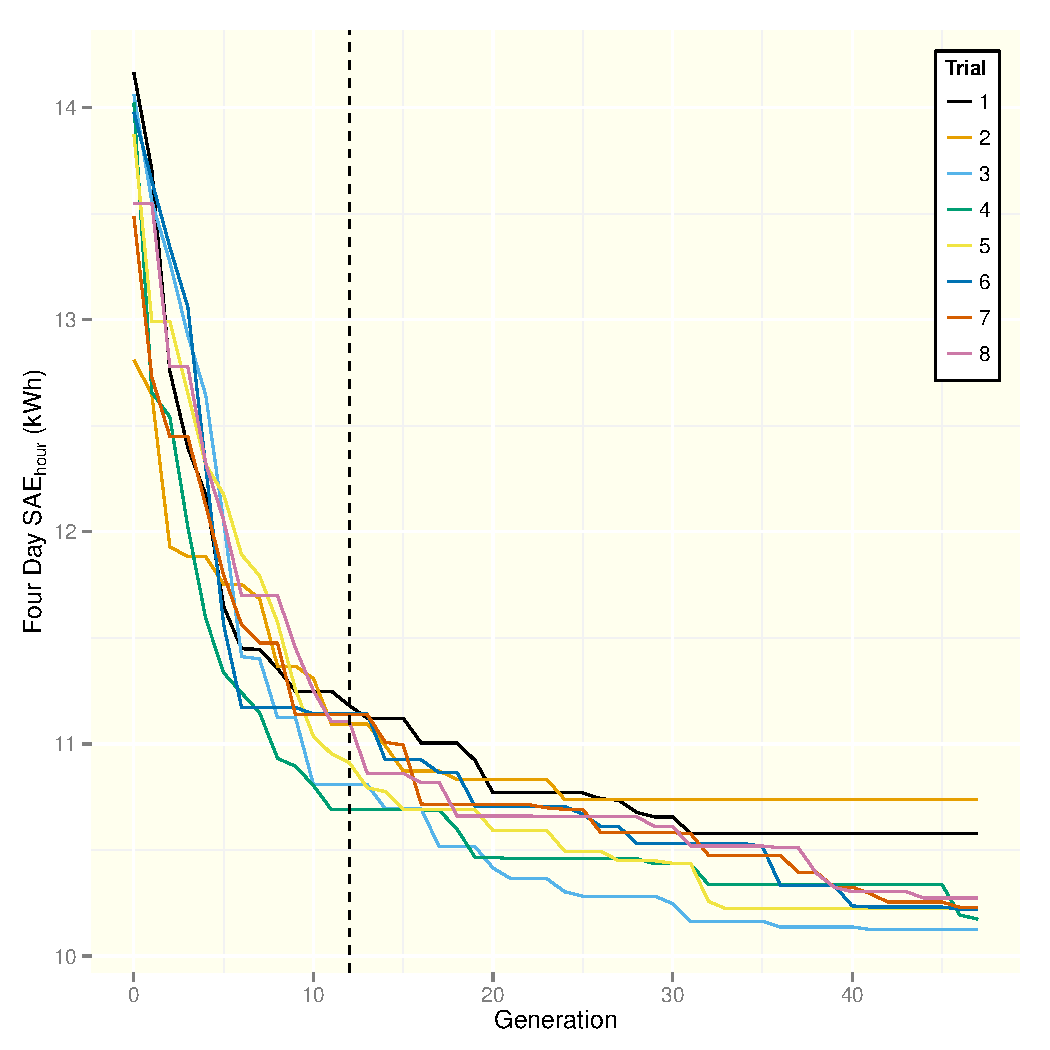
\includegraphics[width=5in]{graphics/figure2.pdf}
\caption{The plot shows the convergence of the best individual in each trial of Experiment 4 when the abbreviated schedule is used (i.e., the first 75\% of the evaluations). The dotted line marks generation 12, which is 25\% of the 1,024 evaluations allotted to the abbreviated schedule. Before this point, individuals produced by the abbreviated schedule tuning are not particularly useful as seeds because of their relatively high SAE.}
\label{fig:hour-converge}
\end{figure}


\section{Conclusions and Future Work}
\label{sec:conclusions}
The results of the previous experiments are summarized in Table~\ref{tab:hourly-summary} and Figure~\ref{fig:hourly-summary}. The table shows the baseline and various approaches for tuning for each model, focusing on the SAE and RMSE between the model output and the actual data. These experiments show that it is possible to use an evolutionary search to reduce the RMSE by over 7\% in a  comparison of hourly electrical usage and that a two-island approach is a feasible, effective way of combining the abbreviated- and full-schedule approaches. 

Experiment 1 verified that a 4 day schedule could serve as a viable surrogate for the full-year schedule in terms of hourly electrical usage, producing a correlation coefficient of 0.96 between abbreviated and full schedules. Experiment 2 showed that an abbreviated-only approach could reduce the RMSE by 6\% and 7\% below the baseline for the refined and primitive models, respectively. Experiment 3 focused on using the full schedule only, which reduced the RMSE by 7\% (refined) and 10\% (primitive). Experiment 4 combined the two approaches in serial fashion, using the abbreviated schedule for the first 768 simulations and then the full schedule for the remaining 256. This approach was better than the abbreviated schedule alone and only slightly worse than the full schedule alone. Experiment 5 combined the two approaches in parallel using an island model, in which one island used the abbreviated schedule and the other the full schedule. This approach was competitive with the full schedule approach, despite using only 25\% of the full-schedule simulations.


\begin{table}[htbp]
\centering
\caption{The summary comparison of results from Experiments 2--5 shows that significant reductions can be gained from tuning with an abbreviated schedule, either alone, serially, or in parallel with full-schedule tuning. Percentages in parentheses are reductions versus the baseline.}
\label{tab:hourly-summary}
\begin{tabular}{lllll}
\toprule
 &  \multicolumn{2}{c}{Refined} & \multicolumn{2}{c}{Primitive}\\
Approach & SAE (kWh) & RMSE & SAE (kWh) & RMSE \\
\midrule
Baseline    & 6242        & 1.206       & 8114        & 1.625 \\\rowcolor{DarkRow}
Abbreviated & 5660 (9\%)  & 1.129 (6\%) & 7453 (8\%)  & 1.514 (7\%)\\
Full        & 5539 (11\%) & 1.119 (7\%) & 7162 (12\%) & 1.458 (10\%)\\\rowcolor{DarkRow}
Serial      & 5581 (11\%) & 1.123 (7\%) & 7343 (9\%)  & 1.497 (8\%)\\
Parallel    & 5597 (10\%) & 1.121 (7\%) & 7270 (10\%) & 1.482 (9\%)\\
\bottomrule
\end{tabular}
\end{table}

\begin{figure}[htbp]
\centering
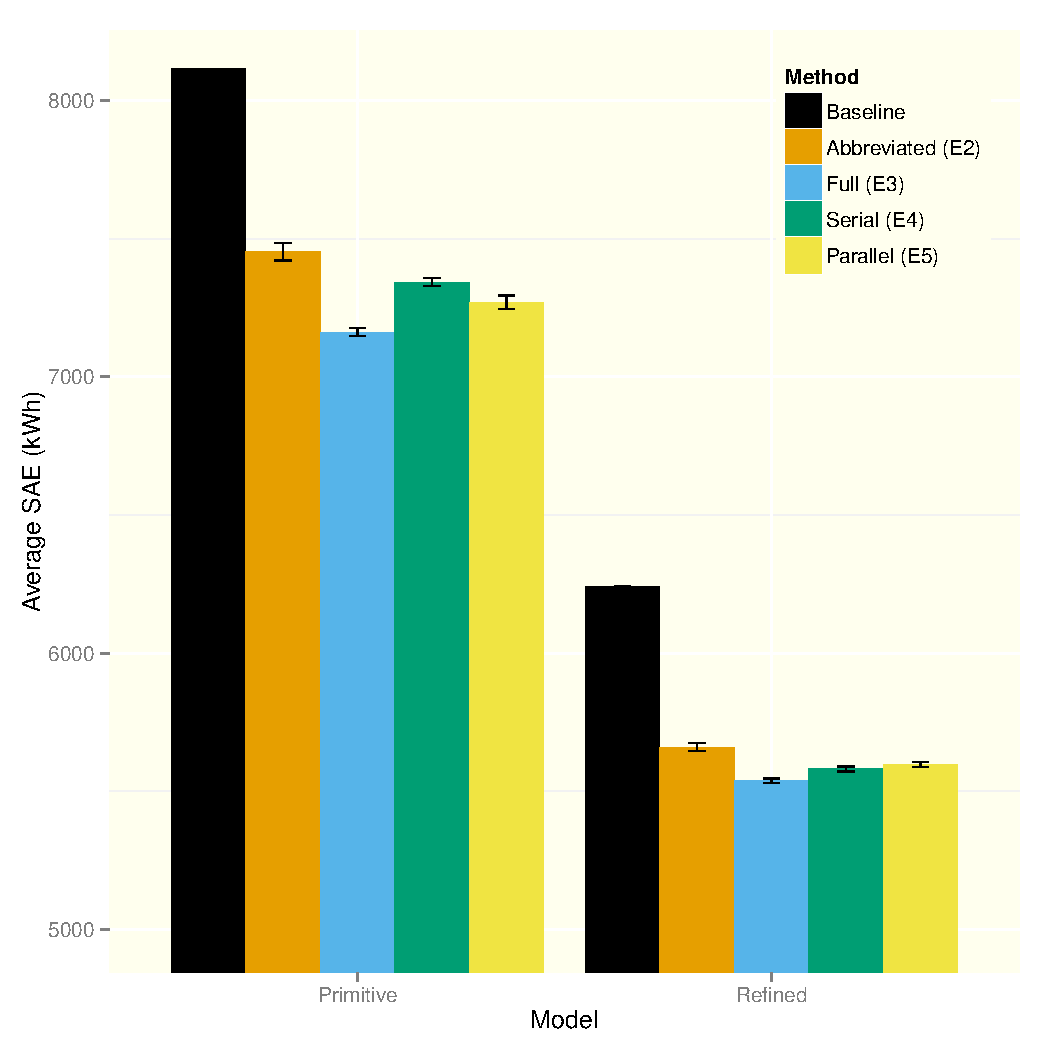
\includegraphics[width=5in]{graphics/figure3.pdf}
\caption{The graph shows the results of Experiments 2--5 compared with the baseline (see Table~\ref{tab:hourly-summary}). The average minimum SAE value found across all eight trials represents each method, and each method is accompanied by standard error bars (except for the baseline). The y-axis minimum value was increased to 5,000 to highlight the differences between the methods.}
\label{fig:hourly-summary}
\end{figure}

The series of experiments elucidates several methods, advantages, and trade-offs in the use of EC to automatically calibrate a software model of an emulated-occupancy experimental residential building to hourly whole-building electrical data. Work is ongoing to extend these calibration methods from % Is ``from'' correct, rather than ``to''? Yes
residential buildings, where fewer things are certain, to larger commercial buildings---calibrating to sub-hourly data for multiple data channels and to quantitative tests for determining not only how closely the building matches measured data but also how accurately the tuned model matches the real building.


\section{Acknowledgements}
This work was funded by field work proposal CEBT105 under DOE Building Technology Activity Number BT0201000. We would like to thank Amir Roth for his support and review of this project. This research used resources of the Oak Ridge Leadership Computing Facility at ORNL, which is supported by the Office of Science of the DOE under Contract No. DE-AC05-00OR22725. Our work has been enabled and supported by data analysis and visualization experts at the RDAV (Remote Data Analysis and Visualization) Center of the University of Tennessee--Knoxville (NSF grant no. ARRA-NSF-OCI-0906324 and NSF-OCI-1136246). ORNL is managed by UT-Battelle, LLC, for DOE under contract DE-AC05-00OR22725. This manuscript has been authored by UT-Battelle, LLC, under Contract Number DEAC05-00OR22725 with DOE. The United States Government retains and the publisher, by accepting the article for publication, acknowledges that the United States Government retains a non-exclusive, paid-up, irrevocable, world-wide license to publish or reproduce the published form of this manuscript, or allow others to do so, for United States Government purposes.


%% The Appendices part is started with the command \appendix;
%% appendix sections are then done as normal sections
%% \appendix

%% \section{}
%% \label{}

%% References
%%
%% Following citation commands can be used in the body text:
%% Usage of \cite is as follows:
%%   \cite{key}          ==>>  [#]
%%   \cite[chap. 2]{key} ==>>  [#, chap. 2]
%%   \citet{key}         ==>>  Author [#]

%% References with bibTeX database:

\bibliographystyle{model1-num-names}
\bibliography{autotune}

%% Authors are advised to submit their bibtex database files. They are
%% requested to list a bibtex style file in the manuscript if they do
%% not want to use model1a-num-names.bst.

%% References without bibTeX database:

% \begin{thebibliography}{00}

%% \bibitem must have the following form:
%%   \bibitem{key}...
%%

% \bibitem{}

% \end{thebibliography}


\end{document}

%%
%% End of file `elsarticle-template-1a-num.tex'.
